\pgfplotsset{compat=1.12}

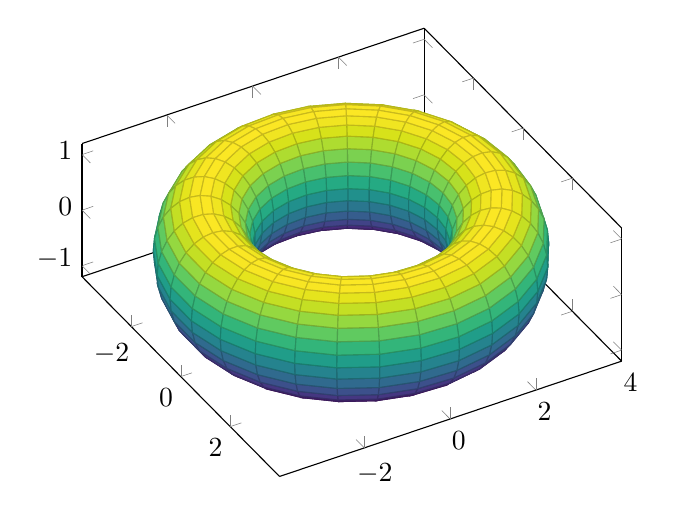
\begin{tikzpicture}
  \begin{axis}[view={60}{60}]
    \addplot3[surf, colormap/viridis, samples = 30, samples y = 30,
              domain=0:2*pi, y domain=0:2*pi, z buffer=sort]
    ({(3+cos(deg(x)))*cos(deg(y+pi/2))}, 
     {(3+cos(deg(x)))*sin(deg(y+pi/2))}, 
     {sin(deg(x))});
  \end{axis}
\end{tikzpicture}

% Taken from here:
% https://tex.stackexchange.com/questions/348/how-to-draw-a-torus
% ...and then modified. I use a different view angle and colormap. To render a partial torus, i.e.
% one that is cut open and missing a piece, one need to restrict the "y domain", for example to
% "y domain=0:2*3*pi/4". The torus takes quite long to compile. It's apparently quite complex.

% When using "samples = 40, samples y = 80", we get the error:
% "TeX capacity exceeded, sorry [main memory size=3000000]."
% 30/60 still works, 35/70 is also too much, 32/64 also works - but only when we render the torus
%  alone - if it's part of a bigger document with more plots, we may get the error again.


